\documentclass{homeworg}
\usepackage{amsmath}

\title{Travail 3 - Circuits équivalents}
\author{Wats Raphaël}

\begin{document}
\maketitle

\section{Schéma du circuit}
    \begin{center}
        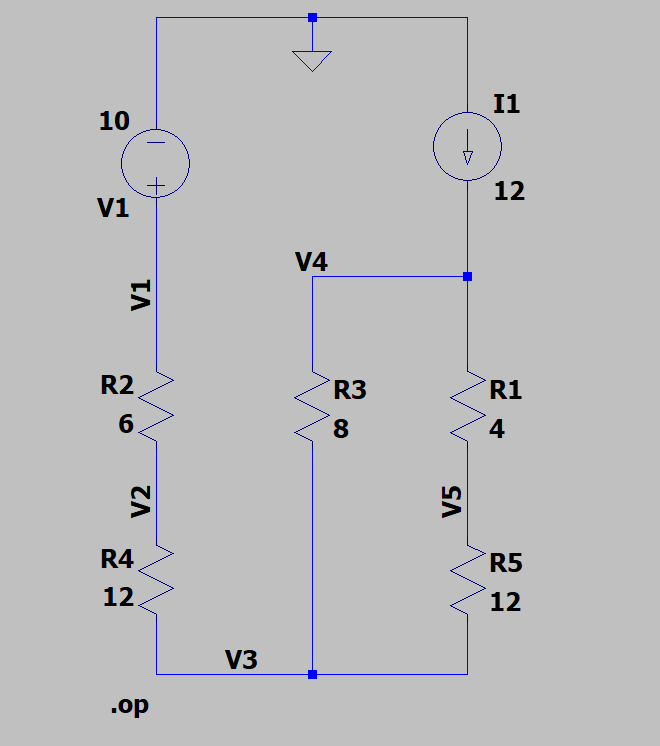
\includegraphics[scale=0.5]{Shematic.png}
    \end{center}

\newpage
\section{Détail des calculs}
    \begin{itemize}
        \item Calcul de la résistance équivalente vu par A et B
            \begin{center}
                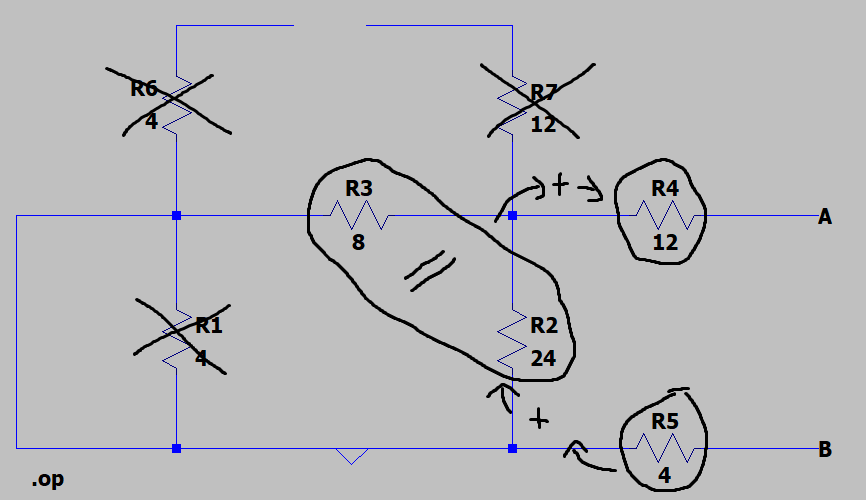
\includegraphics[scale=0.5]{Req.png}
            \end{center}
            Il faut tout d'abord remplacer dans le circuit les sources de voltages par un court-circuit ainsi que les sources de courants par des trous. Pour obtenir $R_e$ on devra simplifier le circuit jusqu'à n'obtenir plus qu'une seule et unique résistance. Comme $R_1$ est court-circuité et que $R_6$ et $R_7$ sont en circuit-ouvert ils n'interviennent pas dans le calcul de la résistance équivalente. On a alors $R_4 + (R_3 // R_2) + R_5$ ce qui nous donne $R_e = 12 + 6 + 4 = 22\Omega$
        \item Calcul de la tension de Thévenin
            \begin{center}
                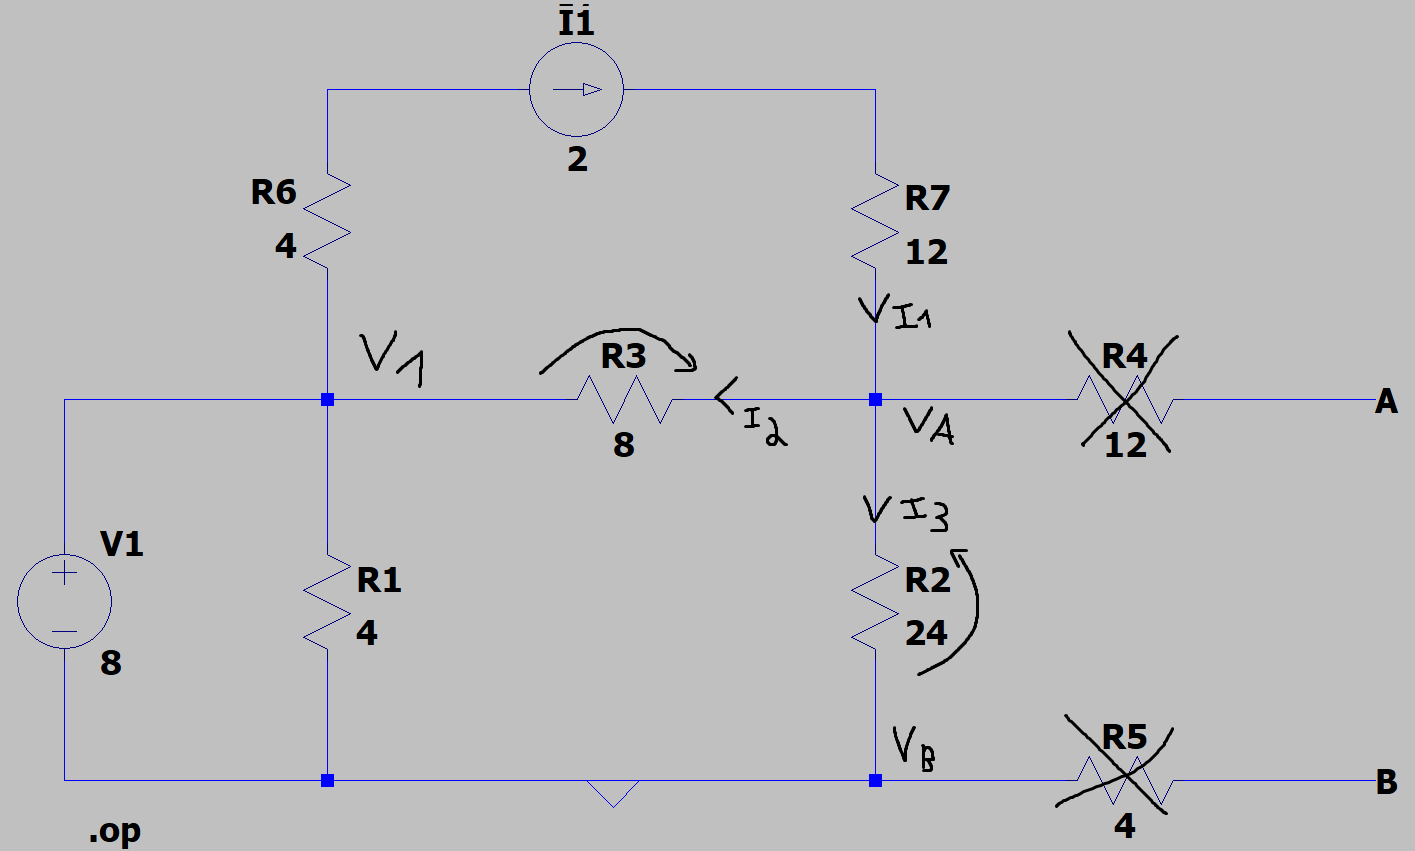
\includegraphics[scale=0.3]{Details.png}
            \end{center}
            \begin{align}
                I_1 = 2\\
                V_B = GROUND = 0\\
                I_1 = I_2 + I_3\\
                I_2 = (V_A - V_1) / R_3 = (V_A - 8) / 8\\
                I_3 = (V_A - V_B) / R_2 = V_A / 24\\
                I_1 = (V_A - 8) / 8 + V_A / 24 = 2\\
                V_A = 18V\\
                V_t = V_A - V_B = 18V\\
                I_n = V_t / R_e = 18/22 = 0,8181818181818182A
            \end{align}
            $V_t$ La tension de Thévenin est égale à la différence de tension entre les bornes A et B on peut alors obtenir le courant de Norton($I_n$) grâce à la relation $I_n = V_t / R_e$.
    \end{itemize}

\section{Simulation}
\begin{itemize}
    \item Simulation du circuit ouvert vérifiant les valeur de $V_A et V_B$ pour la tension de Thévenin.
        \begin{center}
            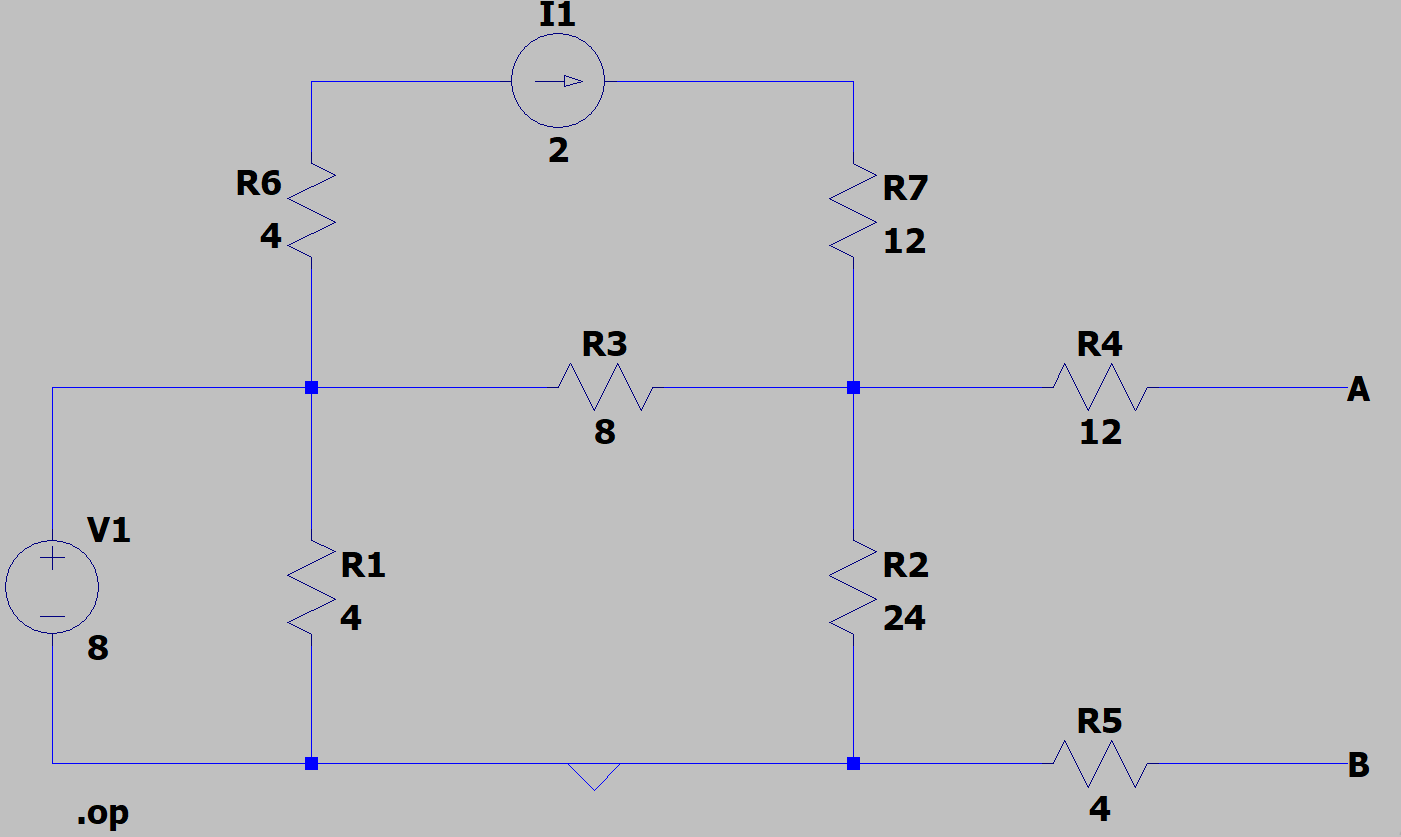
\includegraphics[scale=0.3]{testOpen.PNG}\\
            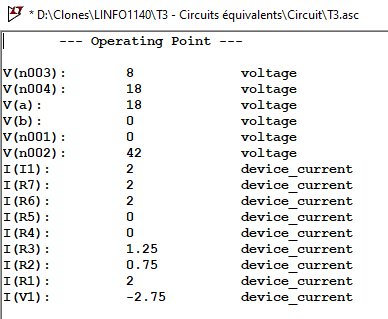
\includegraphics[scale=1]{testOpenSimu.PNG}\\
        \end{center}
    \newpage
    \item Simulation du circuit fermé vérifiant la valeur $R\_test$
        \begin{center}
            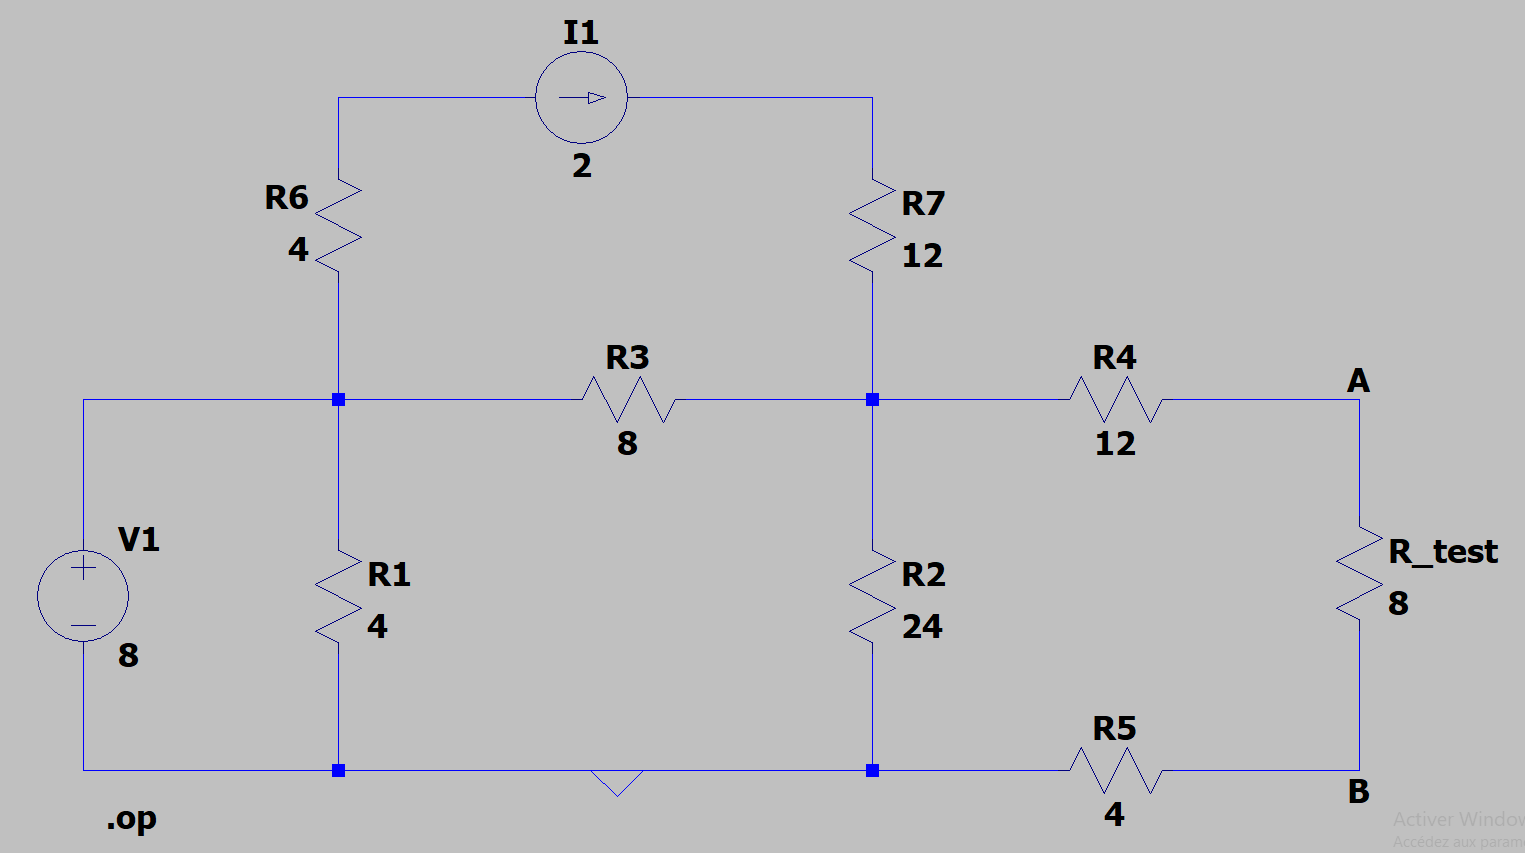
\includegraphics[scale=0.3]{testClose.PNG}\\
            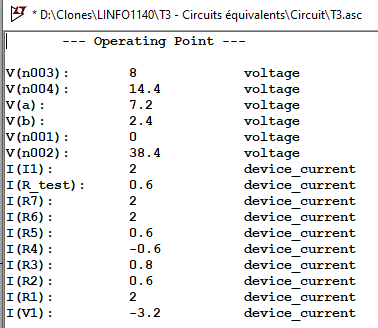
\includegraphics[scale=1]{testCloseSimu.PNG}
        \end{center}
        Ici on peut voir que $I(R\_test)$ est égale à 0.6A et que V(a) - V(b) = 4.8V
        ces valeurs vont nous permettre de vérifier si dans les mêmes conditions de test, les équivalents de Thévenin et Norton produisent les mêmes résultats lors de leur simulation.
    \newpage
    \item Simulation du circuit équivalent de Thévenin:
        \begin{center}
            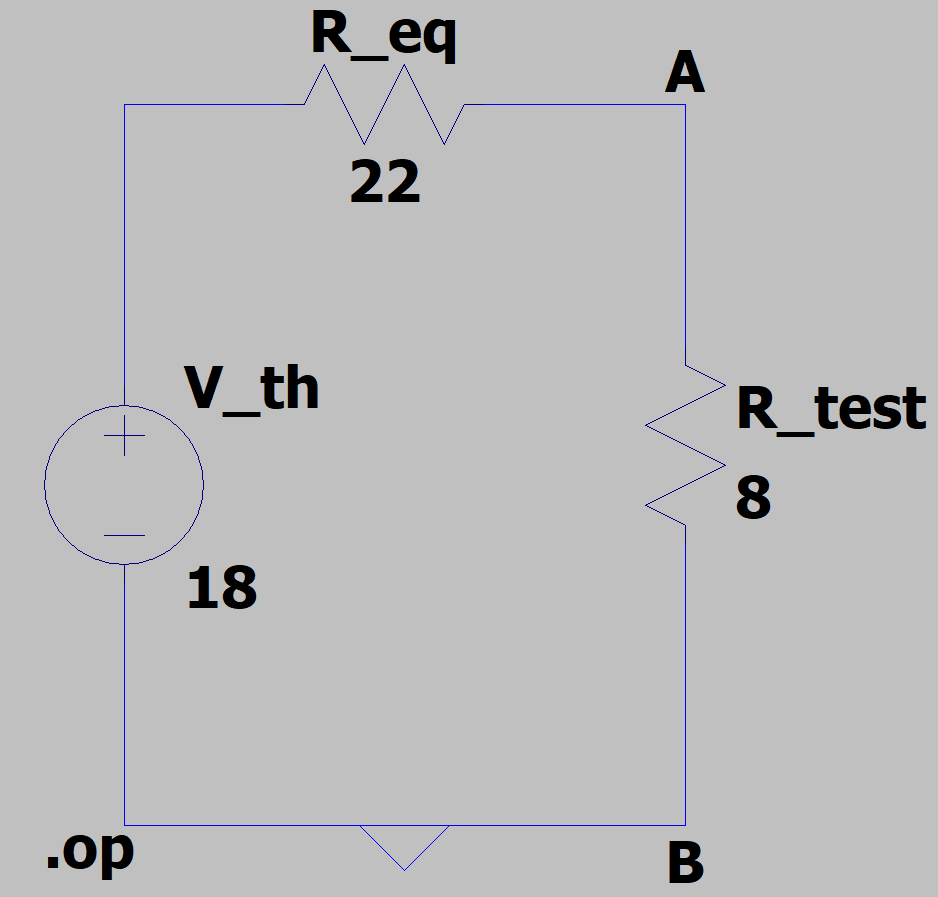
\includegraphics[scale=0.6]{thevenin.png}\\
            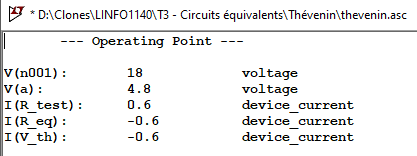
\includegraphics[scale=1]{theveninSimu.png}
        \end{center}
        Le courant de la résistance $I(R\_test)$ est de 0.6A et la tension V(a) est de 4.8V corroborant les résultats obtenu précédemment.
    \newpage
    \item Simulation du circuit équivalent de Norton:
        \begin{center}
            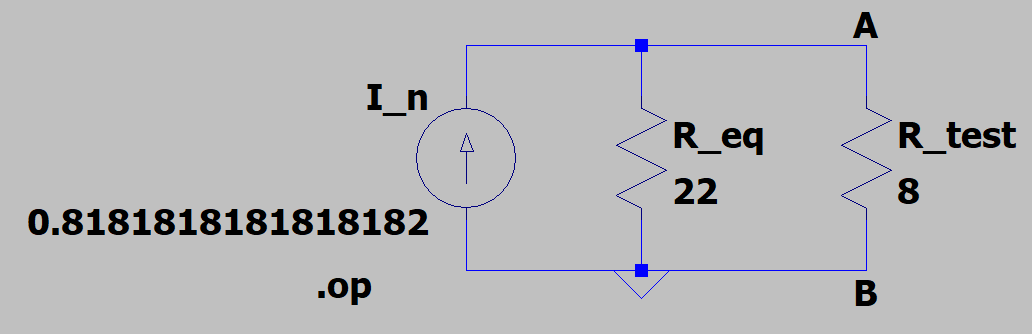
\includegraphics[scale=0.5]{norton.PNG}\\
            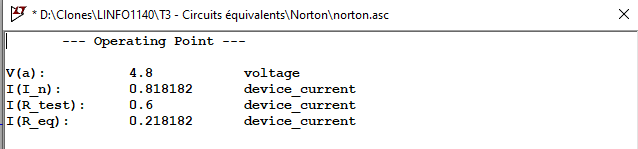
\includegraphics[scale=0.8]{nortonSimu.PNG}
        \end{center}
        Le courant de la résistance $I(R\_test)$ est de 0.6A et la tension V(a) est de 4.8V corroborant une fois de plus les résultats obtenu précédemment.
\end{itemize}


\section{Conclusion}
    Les résultats obtenu sont en adéquation avec ceux obtenu lors de la simulation LTspice XVII.
    \begin{itemize}
        \item Une ou plusieurs résistances parcourues par le même courants sont dîtes en série et leur résistance équivalente sera égale à la somme de celles-ci.
        \item Une ou plusieurs résistance ayant la même différence de tension à leur bornes sont dîtes en parralèle et leurs résistance équivalente sera égale à l'inverse de la somme des inverses de celles-ci.
        \item On peut facilement passez d'un équivalent de Thévenin à un équivalent de Norton et réciproquement.
        \item  Ces théorèmes s'utilisent pour convertir une partie d'un réseau linéaire complexe en un dipôle plus simple.
    \end{itemize}
\end{document}
